\documentclass[11pt,a4paper]{article}
\usepackage[T1]{fontenc}
\usepackage[utf8]{inputenc}
\usepackage{mathptmx}
\usepackage[scaled=0.92]{helvet}
\usepackage{courier}
\usepackage[margin=2.4cm]{geometry}
\usepackage{microtype}
\usepackage{amsmath}
\usepackage{booktabs}
\usepackage{tabularx}
\usepackage{graphicx}
\usepackage{xcolor}
\usepackage{enumitem}
\usepackage[hidelinks]{hyperref}
\setlist{itemsep=2pt,topsep=4pt}
\setlength{\emergencystretch}{3em}

\title{\textbf{JamWarden}: Low-Cost Real-Time Detection of GNSS Jamming\\ and Spoofing with Commodity Receivers}
\author{Varshith\\ \small Blekinge Institute of Technology (BTH), Sweden}
\date{October 2026}

\begin{document}
\maketitle

\begin{abstract}
Jamming and spoofing of global navigation satellite systems (GNSS) around the Baltic Sea now routinely
affect aviation, shipping, and the time synchronisation of critical infrastructure. JamWarden is an open,
low-cost monitor built from an ESP32 microcontroller and a u-blox receiver (about 1{,}000 SEK). It combines
independent indicators from the receiver's RF front end (automatic gain control, noise floor, continuous-wave
interference indicator), from the signal structure (C/N0 level, spread and elevation dependence) and from the
navigation solution (displacement, implied speed, time offset against a local clock). These feed weighted
rules with hysteresis. The same portable C++ detector runs on the microcontroller, in a PC replay tool and
in a reproducible evaluation. On 280 simulated runs (70 hours), JamWarden detected all jamming of 12--25\,dB
and all tested spoofing attacks with median latencies of 2--19\,s and no false alarms in clean, obstructed,
multipath and moving-vessel conditions. A baseline using only the receivers' built-in flags detected
0--65\,\%. Limits are quantified: jammers below about 6\,dB are detected in only 50\,\% of runs, and a
power-matched, elevation-aware spoofer is caught only after it has displaced the position by 50\,m (median
164\,s).
\end{abstract}

\section{Introduction}
GNSS receivers are easy to disrupt because signals arrive at about $-130$\,dBm. A jammer raises the noise
floor so that satellites are lost~\cite{borio}. A spoofer transmits counterfeit signals that capture the
receiver's tracking loops and steer its position or time~\cite{humphreys08,psiaki}. Aviation authorities have
issued repeated safety bulletins about GNSS outages and alterations in the region~\cite{easa}. Professional
interference monitoring uses dedicated hardware, but many affected users (small ports, utilities, schools,
researchers) need a cheap way to know \emph{when} and \emph{where} their GNSS cannot be trusted.

Modern u-blox receivers expose diagnostic data such as AGC count, noise level, a CW jamming indicator and, in
recent generations, a spoofing flag. These indicators are noisy and not always present, and on their own
they cannot separate jamming from a blocked sky. JamWarden's contribution is a transparent detector that
fuses several weak indicators with physical reasoning, together with an open hardware/firmware/dashboard
stack and an evaluation protocol that reports where the approach fails.

\section{Detector}
Every navigation epoch (1\,Hz) the detector computes:
\begin{itemize}
  \item $\bar C$: mean C/N0 of the six strongest satellites; $s_C$: C/N0 standard deviation of satellites
        above 15$^\circ$ elevation (window mean over 10 epochs); $\rho$: Pearson correlation between elevation and
        C/N0 (window median); counts of tracked and strong ($\geq 30$\,dB-Hz) satellites.
  \item From MON-RF (M9/M10) or MON-HW (M8): AGC count, noise per ms, CW jamming indicator, receiver jamming state.
  \item Position displacement from a frozen reference (static mode), implied speed between fixes, altitude
        jumps, the difference between implied and reported speed (mobile mode), and the offset between GNSS UTC
        and the local monotonic clock.
\end{itemize}
A 60\,s baseline (mean and variance) is learned and then adapted slowly ($\alpha = 0.01$) only during clean
epochs. The static reference position is never adapted, which defeats slow drag-off attacks that would
otherwise move it.

\begin{table}[h]
\centering\small
\begin{tabularx}{\linewidth}{@{}l r >{\raggedright\arraybackslash}X@{}}
\toprule
Indicator & Weight & Condition (relative to baseline) \\ \midrule
C/N0 drop & 2.0 & $\bar C_0 - \bar C \geq 6$\,dB or no satellites \\
AGC anomaly & 2.0 & $|AGC - \mu| > \max(4\sigma, 0.1\mu)$ \\
Noise rise / CW indicator & 1.5 / 1.5 & $> \max(4\sigma, 0.2\mu)$ / $> \mu + \max(20, 4\sigma)$ \\
Satellites / fix lost & 1.0 / 1.0 & strong satellites $< 50$\,\% of baseline / no 3D fix \\
Receiver jamming warning / critical & 1.5 / 3.0 & MON-RF/MON-HW jamming state 2 / 3 \\ \midrule
Static displacement / position jump & 3.0 / 3.0 & $> 50$\,m with $h_{acc} < 25$\,m / implied speed $>$ limit (latched 5 epochs) \\
Time jump & 3.0 & $|\Delta$offset$| > 1.5$\,s epoch-to-epoch or vs.\ baseline \\
Receiver spoof flag & 3.0 & NAV-STATUS spoofDetState $\geq 2$ \\
Uniform C/N0 / no elevation dependence & 1.5 / 1.5 & $s_C < 2$\,dB / $\rho < 0.15$ (baseline $\rho > 0.3$) \\
Power rise & 1.0 & $\bar C - \bar C_0 \geq 5$\,dB \\ \bottomrule
\end{tabularx}
\caption{Indicators. Jamming requires score $\geq 3.5$ with at least one RF front-end indicator \emph{and} one
signal-loss indicator. Spoofing requires score $\geq 3$. Alarms need 3 consecutive epochs to raise and 5 to clear.}
\end{table}

The conjunction rule for jamming is the key to robustness: an obstruction (bridge, crane, indoor antenna) also
lowers C/N0 and loses satellites, but leaves the RF front end unchanged. For spoofing, a single-antenna
spoofer produces nearly equal power for all satellites and removes the natural elevation dependence of C/N0
caused by antenna gain and atmospheric path length~\cite{misra}. These are cheap but effective
signal-structure tests.

\section{Implementation}
The detector is portable C++17 without heap allocation in the parsing path (UBX state-machine parser with
checksum verification, decoders, detector). It is tested with 32 unit checks, AddressSanitizer and
UndefinedBehaviorSanitizer. The ESP32 firmware auto-detects the receiver baud rate, configures the needed
messages through CFG-VALSET (M9/M10) or legacy CFG-MSG/CFG-PRT (M8), switches to 115{,}200\,baud and streams
JSON events and status over USB or Wi-Fi. A collector (FastAPI + SQLite) serves a live map with charts and a
GeoJSON export. A physics-inspired scenario generator writes UBX streams with ground truth for 14 scenarios,
including negatives and deliberately hard attacks.

\section{Evaluation}
Each scenario was generated with 20 random seeds (900\,s each, attack onset at 240--360\,s), with the receiver's
own flags randomly present or absent.

\begin{table}[h]
\centering\small
\begin{tabular}{@{}lrrrr@{}}
\toprule
Scenario & JamWarden & Flags only & Median / p90 latency (s) & False alarms \\ \midrule
Broadband jammer, 12--25\,dB & 100\,\% & 50\,\% & 12 / 15 & 0 \\
CW jammer & 100\,\% & 35\,\% & 19 / 24 & 0 \\
Spoofer, drag-off & 100\,\% & 45\,\% & 8.5 / 11 & 0 \\
Spoofer, 30--80\,km jump & 100\,\% & 65\,\% & 2 / 2 & 0 \\
Time shift 2--10\,s (with spoofer) & 100\,\% & 55\,\% & 2 / 2 & 0 \\
Time shift only & 100\,\% & 0\,\% & 2 / 2 & 0 \\
Jam then spoof (40 attacks) & 100\,\% & 45\,\% & 10 / 13 & 0 \\
Vessel, position jump (mobile mode) & 100\,\% & 50\,\% & 2 / 2 & 0 \\
Weak jammer, 4--8\,dB & 50\,\% & 0\,\% & 31.5 / 47 & 0 \\
Power-matched spoofer, 0.3\,m/s & 100\,\% & 45\,\% & 163.5 / 171 & 0 \\
Clean / obstruction / multipath / vessel & -- & -- & -- & 0 \\ \bottomrule
\end{tabular}
\caption{Detection results over 70 simulated hours.}
\end{table}

\begin{figure}[h]
\centering
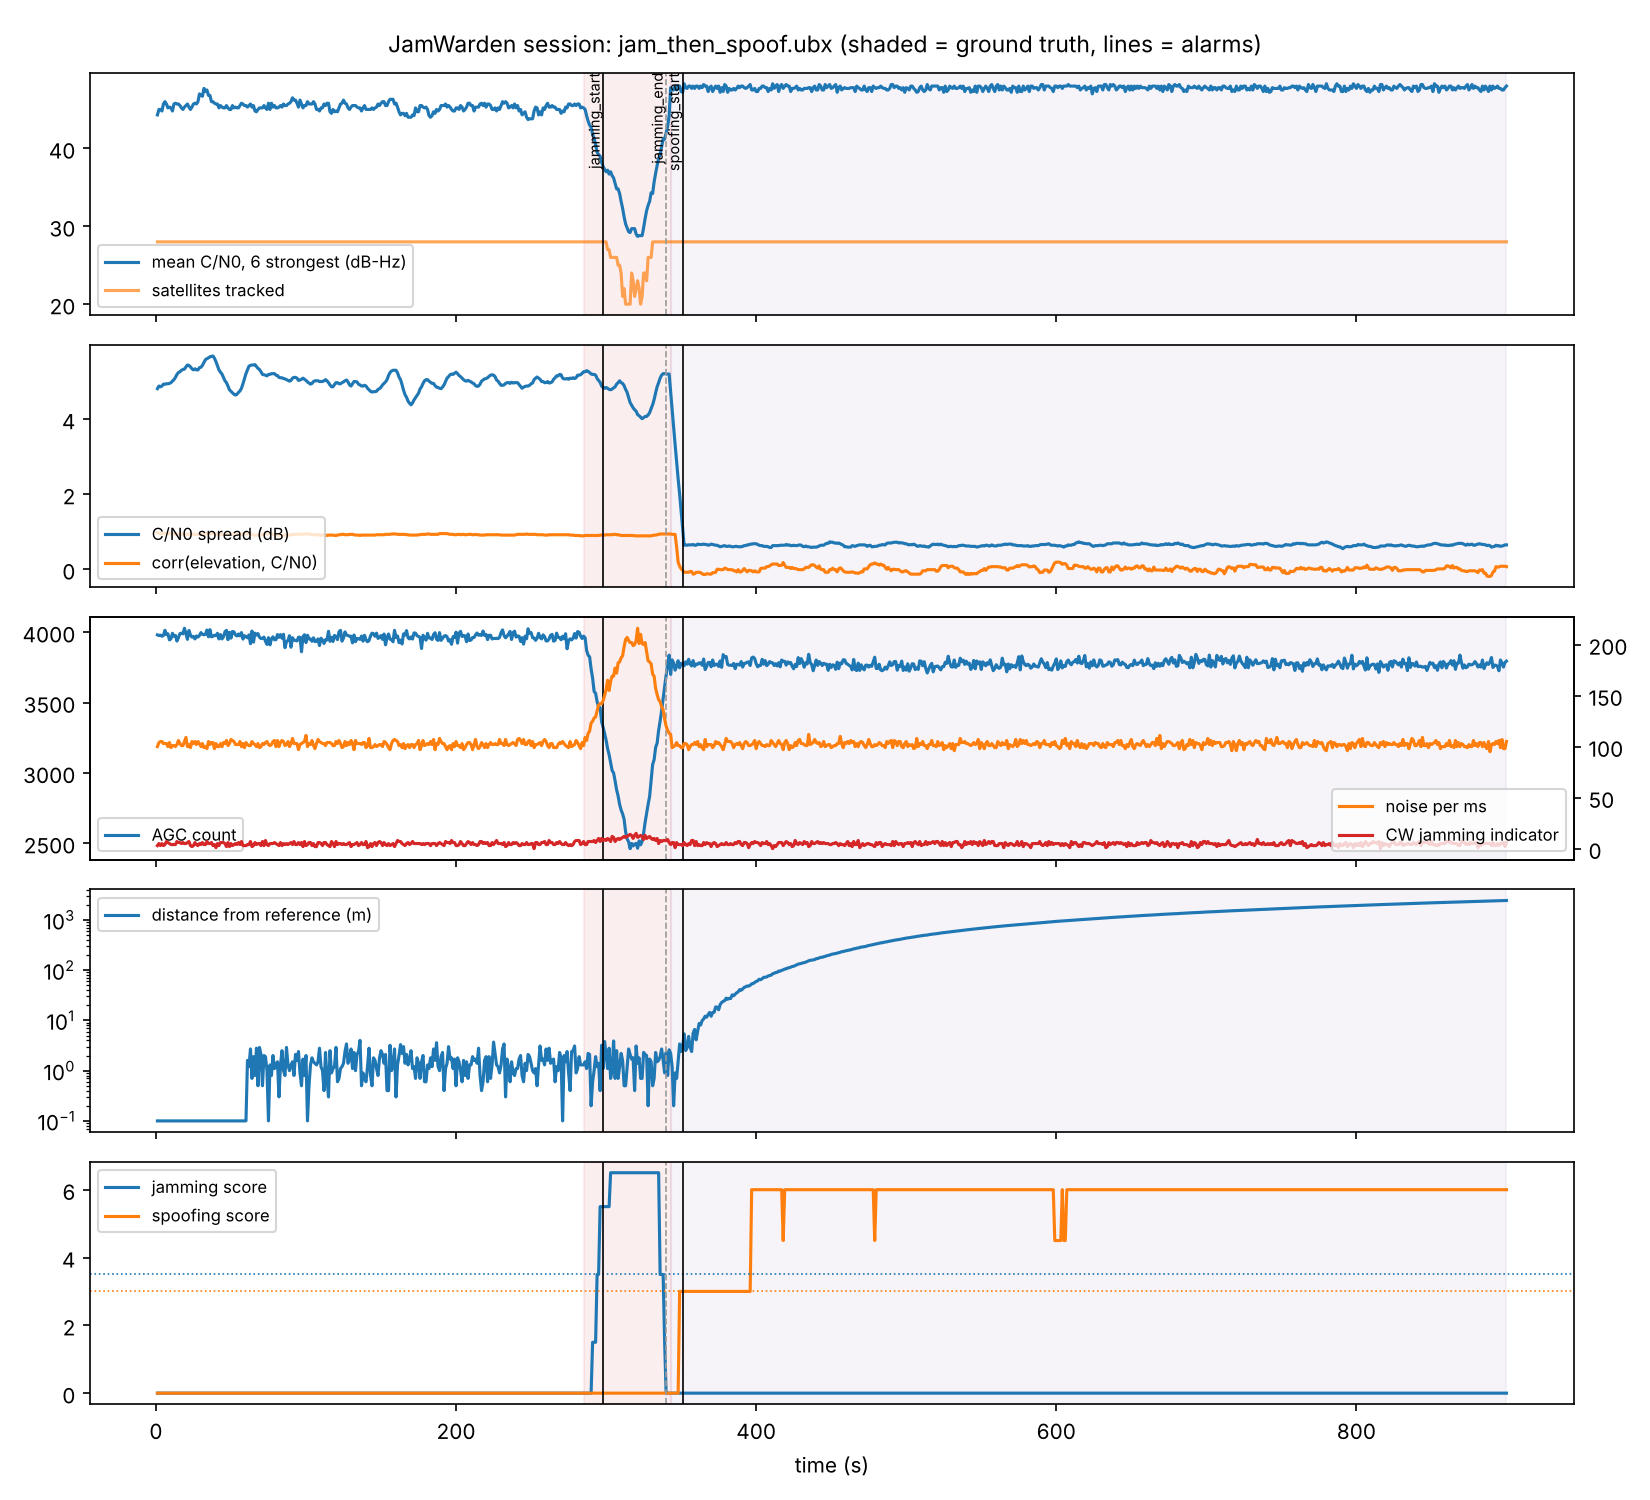
\includegraphics[width=0.92\linewidth]{../docs/session_jam_then_spoof.png}
\caption{Jamming followed by a spoofing takeover. The C/N0 spread and elevation correlation collapse when the
spoofer captures the receiver, before the position starts to move.}
\end{figure}

\paragraph{Discussion.} Fusing independent indicators raises detection well above the receiver's own flags
without false alarms in the negative scenarios. The failures are informative. Jammers that lower C/N0 by
less than the 6\,dB threshold are missed in half of the runs. Lowering the threshold trades directly against
false alarms from ordinary C/N0 variability. A spoofer that imitates power and elevation profiles leaves only
kinematic evidence, so detection waits until the drag exceeds the 50\,m radius. Antenna-array or multi-sensor
techniques such as angle of arrival or cross-sensor consistency~\cite{psiaki} are needed for faster detection.
The evaluation is circular to a degree: the simulator and the detector share physical assumptions. The
results therefore establish correctness and limits, not field performance.

\section{Ethics and legality}
JamWarden is receive-only. Transmitting jamming or spoofing signals is illegal in Sweden and the EU, so
testing relies on simulation, recorded logs, or shielded laboratories. Raw interference data with positions
can reveal sensitive installations, and sharing via the GeoJSON export should be deliberate.

\section{Conclusion and future work}
A 1{,}000\,SEK sensor can detect common jamming and spoofing patterns within seconds by combining RF,
signal-structure, kinematic and timing evidence. Next steps are field recordings in the Baltic region,
validation against public spoofing datasets processed by a software receiver~\cite{texbat}, and multi-sensor
fusion on the dashboard.

\begin{thebibliography}{9}
\bibitem{borio} D.~Borio, F.~Dovis, H.~Kuusniemi, L.~Lo~Presti. ``Impact and Detection of GNSS Jammers on
  Consumer Grade Satellite Navigation Receivers.'' \emph{Proceedings of the IEEE}, 104(6), 2016.
\bibitem{humphreys08} T.~E.~Humphreys, B.~M.~Ledvina, M.~L.~Psiaki, B.~W.~O'Hanlon, P.~M.~Kintner. ``Assessing
  the Spoofing Threat: Development of a Portable GPS Civilian Spoofer.'' \emph{ION GNSS}, 2008.
\bibitem{psiaki} M.~L.~Psiaki, T.~E.~Humphreys. ``GNSS Spoofing and Detection.'' \emph{Proceedings of the IEEE},
  104(6), 2016.
\bibitem{misra} P.~Misra, P.~Enge. \emph{Global Positioning System: Signals, Measurements, and Performance}, 2nd ed.
  Ganga-Jamuna Press, 2006.
\bibitem{texbat} T.~E.~Humphreys, J.~A.~Bhatti, D.~Shepard, K.~Wesson. ``The Texas Spoofing Test Battery: Toward a
  Standard for Evaluating GPS Signal Authentication Techniques.'' \emph{ION GNSS}, 2012.
\bibitem{easa} European Union Aviation Safety Agency. Safety Information Bulletin 2022-02 (and revisions):
  Global Navigation Satellite System Outage and Alterations.
\bibitem{ublox} u-blox AG. u-blox M8, M9 and M10 receiver interface descriptions (UBX protocol).
\end{thebibliography}
\end{document}
